\documentclass{article}
\usepackage{tikz}
\usetikzlibrary{mindmap}

\begin{document}
\pagestyle{empty}

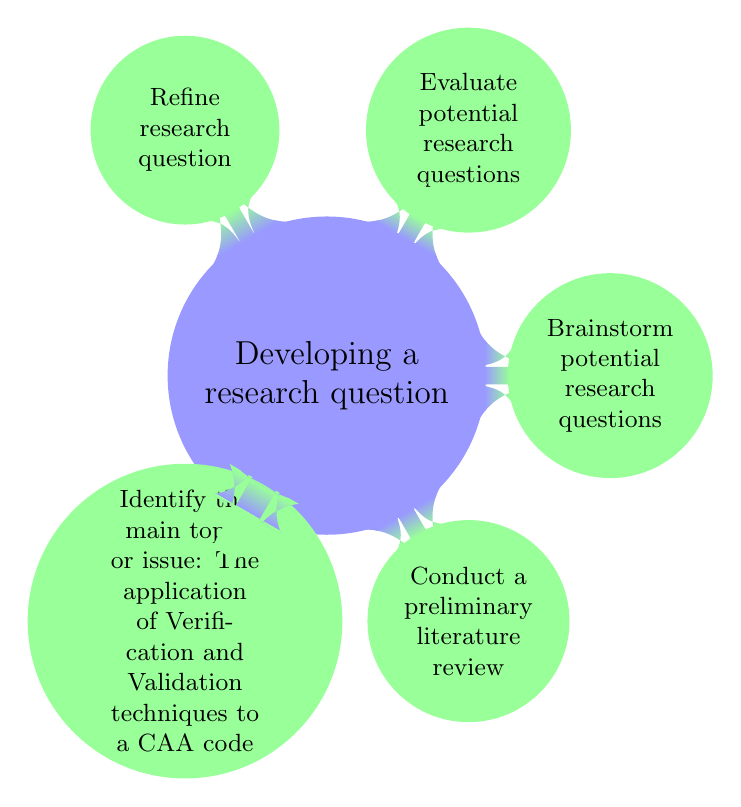
\begin{tikzpicture}[mindmap, grow cyclic, every node/.style=concept, concept color=blue!40, level 1/.append style={level distance=4.5cm,sibling angle=60}, level 2/.append style={level distance=3cm,sibling angle=45}, scale=0.8]

\node{Developing a research question} 
    child [concept color=green!40] { node {Identify the main topic or issue: 
    The application of Verification and Validation techniques to a CAA code }}
child [concept color=green!40] { node {Conduct a preliminary literature review}}
child [concept color=green!40] { node {Brainstorm potential research questions}}
child [concept color=green!40] { node {Evaluate potential research questions}}
child [concept color=green!40] { node {Refine research question}}
;
\end{tikzpicture}

\end{document}

